\section{Numerical Method for Hyperbolic Conservation Laws}\label{se_numerical_method}

\subsection{Notation}
We are interested in solving  hyperbolic conservation laws
\begin{equation} 
\partial_t \bu(x, t) + \partial_x  f(\bu (x, t)) = 0,\quad x \in \Omega \subset \R, t>0,  \\
\label{eq:hpde}
\end{equation}
where  $\bu: \R \times \R \to \R^m$ is the conserved variables and $f$ is the flux function. In this manuscript, we restrict ourself to the one-dimensional setting for simplicity.  In case of a scalar equation, we use additional $u$ instead of $\bu$.
Equation \eqref{eq:hpde} will be later equipped with suitable boundary and initial conditions.
 Since hyperbolic conservation laws may develop discontinuities even for smooth initial data, weak solutions are considered but they are not necessarily unique.
Motivated from physics, one selects the  solution which fulfills the additional 
entropy inequality 
\begin{equation}
\partial_t  U( \bu) + \div F( \bu) \leq 0
\label{eq:eie}
\end{equation}
with convex entropy $U$ and entropy flux $F$. We are working in the framework of FD/FV methods, therefore different kinds of numerical fluxes  are used  in the paper. We denote a general numerical flux of  $f$ with $\fnum$. It has two or more arguments in the following, i.e. 
 $\fnum (\bu_{k-p+1}, \dots, \bu_{k+p})$. 
If we apply an entropy stable flux, e.g. the Godunov flux, we denote this numerical flux by  $g: \R^m \times \R^m \to \R^m$. Using $g$ in a classical  FV/FD methodology results in a low (first) order method. Contrary,  $h: \R^m \times \R^m \to \R^m$ denotes an entropy conservative and 
high-order accurate numerical flux, cf. \cite{tadmor1987numerical, lefloch2002fully}. Please be aware that $g$ and $h$ even without the superscript $\operatorname{num}$ denote always in this paper numerical fluxes. 
The entropy-entropy flux pairs $(U, F)$ are designated using uppercase letters and the notation of  numerical entropy fluxes  are the same as above. It is that the numerical entropy flux $G: \R^p \times \R^p \to \R^p$ is associated with a dissipative numerical flux $g$, analog for $h$. We use further the standard abbreviation, i.e. $g(\bu(x_k, t), \bu(x_{k+1}, t)) = g(\bu_{k}(t), u_{k+1}(t)) = g_{k+\frac 1 2}(t)
$
 generalizing $x_k$ as a way of referring to the center of cell $k$ and $x_{k+\frac 1 2}$  to the right cell boundary, cf. \cref{fig:celldivision}.
 \begin{figure}
			\begin{center}
				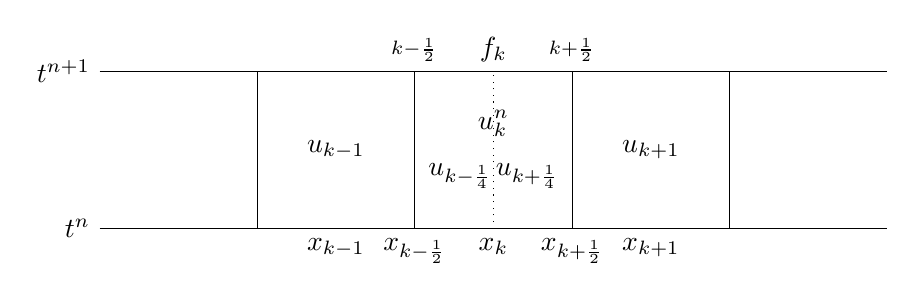
\begin{tikzpicture}
					\draw (-5, 0) -- (5, 0); % n time layer
					\draw (-5, 0) node [left] {$t^n$};
					\draw (-1, 0) -- (-1, 2); % k-1/2 cell boundary
					\draw (-1, 2) node [above]{ $\fnum_{k - \frac 1 2}$};
					\draw (-1, 0) node [below] {$x_{k - \frac 1 2}$};
					\draw (1, 0) -- (1, 2); % k+1/2 cell boundary
					\draw (1, 2) node [above]{ $ \fnum_{k + \frac 1 2}$};
					\draw (1, 0) node [below] {$x_{k + \frac 1 2}$};
					\draw [dotted](0, 0) -- (0, 2); %  k cell division
					\draw (0, 2) node [above] {$f_k$};
					\draw (0, 0) node[below] {$x_k$};
					\draw (-3, 0) -- (-3, 2); %next cell boundaries. 
					\draw (-2, 0) node [below] {$x_{k-1}$};
					\draw (3, 0) -- (3, 2);
					\draw (2, 0) node [below] {$x_{k+1}$};
					\draw (-2, 1) node {$u_{k-1}$};
					\draw (2, 1) node {$u_{k+1}$};
					\draw (0, 4/3) node {$u_k^n$};
					\draw (0, 2/3) node {$u_{k-\frac 1 4}\, u_{k+ \frac 1 4}$};
					\draw (-5, 2) -- (5, 2); % n+1 time layer
					\draw (-5, 2) node [left] {$t^{n+1}$};
				\end{tikzpicture}
				\caption{The subdivision of a cell in space, initialized with the mean value of the old cell.}
				\label{fig:celldivision}
				\end{center}
			\end{figure}
 The same procedure is used for grid points in time in the fully discrete setting, i.e. 
$
  g(\bu(x_k, t_n), \bu(x_{k+1}, t_n)) = g(\bu^n_{k}, \bu^n_{k+1}) = g_{k+\frac 1 2}^n.
$
 Please note that a $2p$ point numerical flux at position $k+ \frac 1 2$ used the points $\bu_{k-p+1}, \dots, \bu_{k+p}$, e.g. for $p=2$ we have 
$
  h(\bu^n_{k-1}, \bu^n_{k}, \bu^n_{k+1}, \bu^n_{k+2}) = h^n_{k+\frac 1 2}.
$
Convex combined numerical fluxes are written as 
 \[
 f_{\alpha_{k+\frac 1 2}}^n = \alpha_{k + \frac 1 2} g^n_{k+\frac 1 2} + \left(1-\alpha_{k+\frac 1 2}\right) h^n_{k+\frac 1 2}.
 \]
%They are depending on $\alpha$ what kind of properties they have, i.e. entropy conservative or dissipative.  
%The position for $\alpha$ also denotes the cell boundary and $\alpha$ is used to differentiate between analytical and convex combination numerical fluxes.
Working with reconstruction free FV methods, the numerical solution in the cell is constant in space at a certain time, in short form i.e. 
$
	f^n_k = f(u^n_k) = f(u(x_k, t_n))
$
for instance. Sometimes cells are cutted in half at position $x_k$ as described in \cref{fig:celldivision}. Therefore  it exists the cell interfaces at $x_{k-1}, x_{k-\frac 1 2}, x_k, x_{k + \frac 1 2}$ and $x_{k+1}$. The middlepoints are  $x_{k-\frac 3 4}, x_{k-\frac 1 4}, x_{k+\frac 1 4}, x_{k+\frac 3 4}$.
We use an uniform mesh with cell length $\Delta x=x_{k+ \frac 12}-x_{k - \frac 12}$ and uniform time-steps $\Delta t= t^{n+1}-t^n$. The mesh ratio is defined by $\lambda= \frac{\Delta t} {\Delta x}$.\\
As mentioned above, to select the physical meaningful solution \eqref{eq:eie} has to be fulfilled.  In terms of our numerical approximation,
the determined solution has been constructed to imitate \eqref{eq:eie} discretely, i.e. in context of first-order FV/FD this means
\[
    \frac{U^{n+1}_k - U^{n}_k}{\Delta t} + \frac{G^n_{k+ \frac 1 2} - G^n_{k-\frac 1 2}}{\Delta x} \leq 0
\]
for an entropy stable numerical entropy flux $G$. 
If the approximated solution satisfies for all entropy pairs such inequality, we call the scheme entropy stable and entropy dissipative if it is only fulfilled for one specific entropy pair. In the last years, many researchers have worked on the construction of entropy conservative and dissipative schemes based either on FD, FV or FE ansatzes, cf. \cite{abgrall2018general, abgrall2021analysis, abgrall2022reinterpretation, chan2018discretely, chen2020review, fisher2013discretely, offner2018stability, ranocha2016summation}. Here, the entropy condition was fulfilled locally.  


\subsection{FV Method with Predictor-Corrector Fluxes}
To explain our blending scheme, we start from the classical FV method.  
A FV method results from integrating the conservation law over a rectangle $\left[x_{k-\frac 1 2}, x_{k + \frac 1 2}\right] \times \left[t^n, t^{n+1}\right]$
\begin{equation} \label{eq:discFVM}
\begin{aligned}
	 u^{n+1}_k =& \int_{x_{k-\frac 1 2}}^{x_{k+\frac 1 2}} \frac{u(x, t^{n+1})}{\Delta x} \vd x \\=& \int_{x_{k+\frac 1 2}}^{x_{k+\frac 1 2}} \frac{u(x, t^n)}{\Delta x} \vd x &+& \frac{1}{\Delta x}\int_{t^n}^{t^{n+1}} f\left(u\left(x_{k-\frac 1 2}, \tau\right)\right) - f\left(u\left(x_{k+\frac 1 2}, \tau \right)\right)  \vd \tau \\
	  \approx&  u^{n}_k &+& \frac{\Delta t}{\Delta x} \left(\fnn_{k-\frac 1 2} - {\fnn_{k+\frac 1 2}}\right).
	 \end{aligned}
\end{equation}
%Some parts of the research community focused on semidiscretisations, i.e. taking the limit $\lim_{t_2 \to t_1} \frac{1}{(t_2 - t_1)}$ in \eqref{eq:discFVM} and using Runge Kutta time discretisations to solve the resulting system of ordinary differential equations \cite{SO1988, SO1989}. 
Taking the limit $\lim_{\Delta t \to 0} \frac{1}{\Delta t}$ in \eqref{eq:discFVM} results in a system of ordinary differential equations (ODEs) which can be solved 
using e.g. Runge-Kutta (RK) schemes \cite{SO1988, SO1989}.  Here, one split between the space and time discretization also referred to as the method of lines ansatz (MOL). If only the PDE is discretized in space, we call the scheme in semi-discrete form.  
 A different approach is based on the assumption that a numerical flux for timesteps $\Delta t=t^{n+1}-t^n$ could be devised based on knowledge of the conservation law and the local time evolution of the solution. 
Based on this line of thought is the Cauchy Kowaleskaya expansion used in \cite{ENOIII} to provide a high-order time-stepping method.  
The drawback of the Cauchy Kowaleskaya approach is that it typically results in lengtly calculations, complex implementations and/or implicit methods where nonlinear solvers are needed. However, we distinguish between the semidiscrete and the fully discrete schemes in the following. 
Obviously, in  \eqref{eq:discFVM} the coupling between neighboring cells has been done via numerical fluxes $\fnn_{k-\frac 1 2}$ to ensure the conservation property. 
A vast amount of numerical fluxes is known in the literature \cite{Lax71, Roe1981, HLL1983, IsmailRoe2009} and even selecting a flux is a nontrivial task \cite{ranocha2018comparison}. Some fluxes, like the Godunov, Lax-Friedrichs, Roe and HLL fluxes, that can be interpreted by exact or approximate Riemann problem solutions, are meant to approximate the flux through some cell boundary over time $\Delta t$, i.e. being the mean value of the flux over this period.  
Numerical fluxes that have only a semidiscrete interpretation need some sort of high order time integration method. 
Our method for high-order time integration is based on a reinterpretation of predictor-corrector time integration \cite[p. 386]{Isaacson1966Analyis} as a numerical quadrature of the numerical flux over a cell boundary.

\begin{theorem}{(Predictor-Corrector-Fluxes)}\label{thm:rkflux}
	Let $\fnum(u_{k}, u_{k+1})$ be a numerical flux and  $u_k(t)$ on $[t, t + \Delta t]$ be the exact solution of the scheme 	\[
	\derd{u_k(t)}{t} + \frac{\fnum(u_{k}(t), u_{k+1}(t)) - \fnum(u_{k-1}(t), u_{k}(t))}{\Delta x} = 0
	\]
	with uniform cell size $\Delta x$.  
	Then, the 4-point numerical flux $\fnum(u_{k-1}, u_{k}, u_{k+1}, u_{k+2})$ defined as
	\[
	\begin{aligned}
	u^1_k =& u_k + \lambda (\fnum(u_{k-1}, u_k) - \fnum(u_{k}, u_{k+1})), \\
	u^1_{k+1} =& u_{k+1} + \lambda (\fnum(u_k, u_{k+1}) - \fnum(u_{k+1}, u_{k+1})), \\
	\fnum(u_{k-1}, u_{k}, u_{k+1}, u_{k+2}) =& \frac{\fnum(u_k, u_{k+1}) + \fnum\of{u^1_{k}, u^1_{k+1}}}{2}
	\end{aligned}
	\]
	is a second-order\footnote{Please note that the term $p$ order accurate was coined so that integration via a $p$ order quadrature rule leads to a $p$ order accurate approximation.} accurate approximation of
$
		\frac{1}{\Delta t}\int_{t}^{t + \Delta t} \fnum(u_{k}(\tau), u_{k+1}(\tau)) \vd \tau,
$
	i.e.
	\[
		\norm{\fnum(u_{k-1}, u_{k}, u_{k+1}, u_{k+2}) - \frac{1}{\Delta t}\int_{t}^{t + \Delta t} \fnum(u_{k}(\tau), u_{k+1}(\tau)) \vd \tau} = \mathcal O{(\Delta t)^2}.
	\]
	\begin{proof}
		We begin by stating that the intermediate values $u^1_{k}, u^1_{k+1}$ are first-order accurate, i.e. 
		\[
		u^1_{k} = u_k(t + \Delta t) + \mathcal O\of{(\Delta t)^2} \quad u^1_{k+1} = u_{k+1}(t + \Delta t) + \mathcal O\of{(\Delta t)^2}
		\]
		due to the explicit Euler method. Calculation of the flux between cell $u_k$ and $u_{k+1}$ over time $\Delta t$ via the trapezoid rule $\nquad$ (second-order) and the exact solution $u_k(t)$ is second-order accurate, i.e.
		\[
		\begin{aligned}
		\nquad[\fnum(u_{k}(\cdot), u_{k+1}(\cdot))] = &\frac{\Delta t}{2}(\fnum(u_k(t), u_{k+1}(t)) + \fnum(u_{k}(t + \Delta t), u_{k+1}(t+ \Delta t))) \\ = &\int_t^{t + \Delta t} \fnum(u_{k}(\tau), u_{k+1}(\tau))\vd \tau + \mathcal O\left((\Delta t)^3\right).
		\end{aligned}
		\]
	%	as the trapezoid rule is second-order accurate. 
		Due to the Lipschitz continuity of $\fnum$, we have 
		\[
		\norm{\fnum(u_l(t + \Delta t), u_r(t + \Delta t)) - \fnum(u^1_l, u^1_r)}\leq L_f \left(\norm {u_l(t + \Delta t) - u^1_l} + \norm{u_r(t + \Delta t) - u^1_r}\right),
		\]
		where $u_l$ and $u_r$ denote the left and right value at some generic interface. 
	Due to the accuracy order of $u^1_k$ and $u^1_{k+1}$, it follows
		\[
			\norm{\fnum(u_k(t + \Delta t), u_{k+1}(t + \Delta t)) - \fnum(u^1_k, u^1_{k+1})} = \mathcal O\left(\Delta t^2 \right).
		\]
		The combination of these three statements yields that the numerical quadrature of the flux calculated using the approximate values $u^1_k, u^1_{k+1}$
		\[
		\begin{aligned}
		\Delta t \fnum 	=& \frac{\Delta t }{2}(\fnum(u_{k}, u_{k+1}) + \fnum(u^1_k, u^1_{k+1})) \\
						=& \frac{\Delta t }{2}(\fnum(u_k, u_{k+1}) + \fnum(u_k(t + \Delta t), u_{k+1}(t + \Delta t)) + \mathcal O(\Delta t)^2) \\
						=& \nquad[\fnum(u_k(\cdot), u_{k+1}(\cdot))] + \mathcal O(\Delta t)^3 \\
						=& \int_t^{t + \Delta t} \fnum(u_k(\tau), u_{k+1}(\tau))\vd \tau + \mathcal O\left(\Delta t^3\right) 
		\end{aligned}
		\]
		is a second-order exact approximation and dividing by $\Delta t$ induces the result.
		\end{proof}
\end{theorem}
The above numerical flux $\fnum(u_{k-1}, u_{k}, u_{k+1}, u_{k+2})$ could be also interpreted as the flux over the given cell boundary if the semidiscrete scheme is used together with the strong stability preserving (SSP) RK(2,2) method which is equivalent to the deferred correction method of order 2 \cite{abgrall2021relaxation}. However, higher-order quadrature rules can also be applied in this context. 
%\begin{remark}[Connection to classical RK-FV methods and Variation of the Time Integration Method]
%	The above numerical flux $\fnum(u_{k-1}, u_{k}, u_{k+1}, u_{k+2})$ could be also interpreted as the flux over the given cell boundary if the semidiscrete scheme is used with the SSPRK(2,2) time integration method, but other quadrature/integration methods are possible. In case strong stability preserving Runge-Kutta methods are used together with an entropy dissipative/stable flux the constructed flux will be also entropy dissipative/stable with entropy flux given by
%	\[
%		\Fnum(u_{k-1}, u_k, u_{k+1}, u_{k+2}) = \frac{\Fnum(u_k, u_{k+1}) + \Fnum(u^1_{k},u^1_{k+1})}{2}.
%	\]
%	\end{remark}
%
%\todo{Um ehrlich zu sein,  macht das hier etwas wenig Sinn... Es kommt nicht raus was du ausdrücken willst. Ich glaube ich weiß es aber halte es für komplett unverständlich... Darüber müssen wir am Freitag unbeidngt reden. }
To describe now the method, we follow  \cite{klein2021using} where the considered blending FV scheme has been proposed. The method  fulfills  Dafermos' entropy condition   \cite{dafermos1973entropy} as defined like follows: 
\begin{definition}[Dafermos' Criteria]\label{def_Dafermos}
Let $\bu$ be a weak solution of \eqref{eq:hpde} and $U$ an entropy. The total entropy in the domain  $\Omega$ is given by 
\[
E_\bu(t) = \int_{\Omega} U( \bu(x, t)) \vd x.
\]
A Dafermos entropy solution $\bu$ is a weak solution that satisfies 
\begin{equation}\label{eq_Dafermos}
 \forall t > 0: \quad \partial_t E_\bu(t) \leq \partial_t E_{\tilde{\bu}}(t) 
\end{equation}
compared to all other weak solutions $\tilde \bu$ of the conservation law \eqref{eq:hpde}. In essence, the entropy of the selected solution decreases faster than the entropy of all other solutions.
\end{definition}
%To describe the scheme from \cite{klein2021using}, we select the scalar setting in  \eqref{eq:hpde}. 

\begin{definition}\label{def_Blending}
The blending scheme is based on the FV approach in conservative form. Instead of using classical numerical fluxes in 
\eqref{eq:discFVM}, a convex combination between classical Godunov-type flux  and  a high-order entropy conservative flux  is used instead. 
The combined flux, called GT-flux, is given by
	\begin{equation}\label{eq_GT_flux}
     f_{\alpha_{k+\frac 1 2}}^n := \alpha_{k + \frac 1 2} g^n_{k+\frac 1 2} ( {\bu_k,\bu_{k+1}}) + (1-\alpha_{k+\frac 1 2}) h^n_{k+\frac 1 2} (\bu_{k-p+1}, \dots, \bu_{k+p})
     	\end{equation}
	where $\alpha_{k+\frac 1 2} \in [0,1]$ is the convex parameter. 
\end{definition}
\begin{example}
To give a concrete example, using the explicit Euler method for the time,  the scheme is given by 
\begin{equation}\label{eq_Scheme}
\bu^{n+1}_i =\bu^{n}_i + \frac{\Delta t}{\Delta x} \left(  f_{\alpha_{k+\frac 1 2}}^n   - f_{\alpha_{k-\frac 1 2}}^n  \right).
\end{equation}
To obtain higher order in time, RK methods can be used instead, which can be rewritten into the fluxes as described in  \cref{thm:rkflux} yielding a high-order method that can be written with explicit Euler steps. Please be aware, that also different time-integration methods can be combined for the convex combination resulting in highly efficient schemes using  \cref{thm:rkflux}.
\end{example}
The properties of the scheme highly depend on the selected fluxes and  on the convex parameter $\alpha_{k+\frac12}$.
The value of $\alpha_{k+\frac12} = \alpha (\bu_{k-p+1}, \dots, \bu_{k+p})$ itself depends on $\bu_i$ %Therefore the properties of the flux will depend on the selected function $\alpha_{k+\frac12} $ 
which takes the high-order stencil into account.
Before we repeat how $\alpha$ has to be selected to ensure that our scheme fulfills additionally Dafermos' criteria \eqref{eq_Dafermos}, we want to summarize the following  basic properties of the scheme and the numerical fluxes:
\begin{itemize}
\item The GT-flux is consistent and local Lipschitz continuous \cite[Lemma 1]{klein2021using}. 
\item The GT-flux with Tadmor's entropy conservative flux or the high-order modification from \cite{lefloch2002fully} satisfies as well the semidiscrete cell entropy inequality locally for the selected entropy pair used in the construction of the flux for all $\alpha  \in (0, 1]$ \cite[Theorem 1]{klein2021using}.
\item Due to the conservation form of \eqref{eq_Scheme} and the convex combination of the flux, the scheme is locally conservative and the Lax-Wendroff theorem is valued due to the applications of the results from \cite{shi2018local}.
\end{itemize}
As we mentioned before, the parameter $\alpha$ is essential for the properties of the underlying method and we repeat from \cite{klein2021using} the following definition:
\begin{definition}
	We call $\alpha: \R^{2p\times m} \to [0, 1]$ an entropy inequality predictor with a $(2p)$ point stencil if
	\begin{align*}
&\lim_{\Delta x \to 0}	\alpha(u_{k-p+1}, \dots, u_{k +p}) \\ = &\begin{cases} 0 &  \exists x \in [x_k -(p-1)\Delta x, x_k + p\Delta x]: \derive{U}{t} + \derive{F}{x} < 0\\
	1 & \forall x \in [x_k -(p-1)\Delta x, x_k + p\Delta x]:\derive{U}{t} + \derive{F}{x} = 0 \end{cases}
	\end{align*}
	holds for the complete stencil. We will call the entropy inequality predictor slope limited if 
	\[ \abs{\alpha_k - \alpha_{k+1}} < M \quad \text{with} \quad \alpha_k = 	\alpha(u_{k-p+1}, \dots, u_{k+p} )\]
	holds for some $M < 1$ and all $i$.
\end{definition}
In \cite{klein2021using}, a slope entropy inequality predictor was constructed starting from Godunov-type flux and demonstrated  that it is slope limited. The predictor is given by 
	\begin{equation}\label{eq_predictor}
	\alpha^n = H_{sm}\left( \frac{\frac {s^n_k}{s_{ref}} -a}{b}   \right) \circledast \hat{h},
	\end{equation}
where $s^n_k$ is the entropy dissipative rate from the classical Godunov scheme
	\begin{equation*}
		s^n_k(t) = \frac{G\of{u^n_{k+1}, u^n_{k}} - G\of{u^n_k, u^n_{k-1}}} { \Delta x} + \frac{U\of{u_k^{n+1}} - U\of{u^{n}_{k}}} { \Delta t}.
	\end{equation*}
 $s_{ref}$ its  minimum value, $\hat{h}$ the cut hat function ($h(x)=\max(0,\min(1,2x+2,-2x+2)$), $H\in C^2$ the smothstep function  
		\begin{equation*}
			H_{sm}(x) = \begin{cases}
				0 & x  \leq 0 \\
				6x^5 - 15x^4+10x^3 & 0 \leq x  \leq 1\\
				1 & 1 \leq x, \\
			\end{cases}
		\end{equation*}
and $\circledast $ denotes the discrete sup-mollification 
$
		(f \circledast g)|_{[i/n, (i+1) / n]} = \max_{j \in \{0, \dots, n-1\}} f_j g_{i-j}$ for $ i = 0, \dots, n-1
$
and step functions $f,g$. 
\begin{remark}
Instead of working with the classical Godunov flux in \cref{def_Blending}, we  use approximated Riemann solvers. In \cite{klein2021using}, the local Lax-Friedrich flux  (LLF) (Rusanov) has been used and shows promising results. In the numerical section, we apply always the LLF flux to obtain a more efficient method. 
Finally, we like to point out that extension of the method to two dimension is straightforward via a tensor-structure ansatz. All of our now considered results can be transferred. 
\end{remark}

\subsection{Local entropy inequality}\label{subsec_local_entropy}
Here, we want to extend the investigation of  \cite{klein2021using} and demonstrate that the method satisfies locally a fully discrete entropy inequality 
%
%A noteworthy fact is that a scheme constructed using this methodology satisfies a discrete entropy inequality 
under additional restrictions on $\alpha$. We  define the entropy production of the semidiscretly entropy conservative flux scheme
\[
	p^n_k = \frac{H\of{u_{k - p+1}, \dots, u_{k+p}} - H\of{u_{k-p+1}, \dots,  u_{k+p}}}{\Delta x} + \frac{U\of{u^{n+1}_k} - U \of {u^n_k}}{\Delta t}
\] 

and call  \textbf{Condition $F$}  the following:
\begin{definition}
	The parameter $\alpha$ is said to satisfy \textbf{Condition $F$} for cell $k$ if
\[
	\alpha_{k+\frac 1 2} s^n_{k + \frac 1 4} + \left(1-\alpha_{k + \frac 1 2}\right) p^n_{k + \frac 1 4} \leq 0 \text{ and }  \alpha_{k-\frac 1 2} s^n_{k - \frac 1 4} + \left(1-\alpha_{k - \frac 1 2}\right) p^n_{k - \frac 1 4} \leq 0
\]
	holds for the left and right cell interfaces.
\end{definition}
We can prove: 
\begin{lemma}\label{lem:EalpBound}
	\textbf{Condition $F$} is fulfilled for cell $k$ if one of the following conditions is satisfied on each cell interface, i.e. for $k+\frac 1 4$ and $k-\frac 1 4$.
	\begin{enumerate}
		\item It holds $s^n_{k+\frac 1 4} \leq 0$ and $p^n_{k+\frac 1 4} \leq 0$, $\alpha \in [0, 1]$ is arbitrary.
		\item It holds $s^n_{k + \frac 1 4} \leq 0$ and $p^n_{k + \frac 1 4} > 0$ and $\alpha \geq \frac{p^n_{k+\frac 1 4}}{p^n_{k + \frac 1 4} - s^n_{k + \frac 1 4}}$.
	\end{enumerate}
	\begin{proof}
		The first condition is obvious. For the second one the following calculation
		\[
			\alpha s + (1-\alpha) p \leq 0 \iff \alpha(s-p) + p \leq 0 \iff  \alpha \geq \frac{p}{p-s} \geq 0
		\]
		with suppressed indices show the result. Please note that $s-p < 0$ holds by construction.
		\end{proof}
	\end{lemma}
	The aforementioned result allows to calculate a lower bound on $\alpha$ to enforce  \textbf{Condition $F$} if one can guarantee that $s^n_{k+\frac 1 4} > 0$ never happens. As the Godunov flux or Lax-Friedrichs flux are two entropy stable examples  the case $s^n_{k + \frac 1 4}>0$ never happens if an appropriate CFL condition is minded. The following theorem is based on \cite{Tadmor84II} and \cite{klein2021using}:
\begin{theorem}\label{thm:deie}
	The discrete GT-Scheme satisfies a discrete per cell entropy inequality with the flux
	\[
	\Fnum(u_{k-p+1}, \dots, u_{k+p}) = \alpha_{k+\frac 1 2} G(u_{k-p+1}, \dots, u_{k+p}) + (1-\alpha_{k+\frac 1 2}) H(u_{k-p+1}, \dots, u_{k+p}) 
	\]
	if $\alpha_{k+\frac 1 2}$ fulfills the condition $F$ for both cell boundaries and the CFL restriction is half that of the minimum of either fluxes. 
\end{theorem}
		\begin{proof}
	
	We first state that the cell mean $u^{n+1}_k$ can be written as the average value 
	\[
	\begin{aligned}
	u^{n+1}_k 
	=& u^n_k + \lambda \left (\fnn_{\alpha_{k-\frac 1 2}} - \fnn_{\alpha_{k+\frac 1 2}} \right) \\
	=& \frac{u^n_k + 2 \lambda \left(\fnn_{\alpha_{k-\frac 1 2}} - f\of{u^n_k} \right) + u^n_k + 2 \lambda \left(f\of{u^n_k}-f^n_{\alpha_{k+\frac 1 2}} \right) } {2} 
	\\
	=& \frac{\alpha_{k-\frac 1 2} \left (u^n_k + 2 \lambda \left(g^n_{k-\frac 1 2} - f\of{u^n_k} \right) \right) 
	+ \left(1- \alpha_{k-\frac 1 2} \right)\left(u^n_k + 2 \lambda \left(h^n_{k-\frac 1 2} - f\of{u^n_k} \right)\right) }{2}\\
	&+ \frac{\alpha_{k+\frac 1 2} \left(u^n_k + 2 \lambda \left(f\of{u^n_k}-g^n_{k+\frac 1 2} \right)\right) 
	+ \left(1-\alpha_{k+\frac 1 2}\right)\left(u^n_k + 2 \lambda \left(f\of{u^n_k}-h^n_{k+\frac 1 2} \right) \right) } {2} \\
	=& \frac{u^{n+1}_{k-\frac 1 4} + u ^{n+1}_{k+\frac 1 4}}{2}
	\end{aligned}
	\]
	of two schemes and therefore one concludes that for the entropy of cell $k$ holds 
	\begin{equation}
        \begin{aligned}
		&U(u^{n+1}_k) - U(u^n_k) + \lambda (\Fnn_{\alpha_{k+\frac 1 2}} - \Fnn_{\alpha_{k - \frac 1 2}}) \\
		\leq &
		 \frac {U\of {u^{n+1}_{k-\frac 1 4}} + U \of {u^{n+1}_{k+\frac 1 4}} }{2} - U\of{u^n_k} + \lambda \left( \Fnn_{\alpha_{k+\frac 1 2}} - \Fnn_{\alpha_{k - \frac 1 2}}\right)\\
		= &
		\frac{U\of {u^{n+1}_{k-\frac 1 4}} - U \of{u^n_k} + 2 \lambda \left( F^n_{k} - \Fnn_{\alpha_{k - \frac 1 2}}\right)}{2} 
		+ \frac{U\of {u^{n+1}_{k+\frac 1 4}} - U \of{u^n_k} + 2 \lambda \left( \Fnn_{\alpha_{k+\frac 1 2}} - F^n_{k} \right)}{2} \\
		\leq & \frac{\alpha_{k-\frac 1 2}}{2}\left(U \left(u^n_k + 2 \lambda \left(g^n_{k-\frac 1 2}-f\of{u^n_k} \right) \right) - U(u^n_k) + 2 \lambda  \left( F^n_{k} -G^n_{k-\frac 1 2} \right) \right) \\ 
		&+ \frac{1-\alpha_{k-\frac 1 2}}{2} \left(U\of{u^n_k + 2 \lambda \left(h^n_{k-\frac 1 2}-f\of{u^n_k} \right)}  -U(u^n_k) + 2 \lambda  \left(F^n_{k} - H^n_{k-\frac 1 2} \right) \right) \\
		&+ \frac{\alpha_{k+\frac 1 2}}{2}\left(U \of{u^n_k + 2 \lambda \left(f\of{u^n_k}-g^n_{k+\frac 1 2} \right)} - U(u^n_k) + 2 \lambda   \left(   G^n_{k+\frac 1 2} - F^n_{k}\right) \right) \\ 
		&+ \frac{1-\alpha_{k+\frac 1 2}}{2} \left(U\of{u^n_k + 2 \lambda \left(f\of{u^n_k}-h^n_{k+\frac 1 2} \right)} - U(u^n_k) + 2 \lambda  \left(  H^n_{k+\frac 1 2} - F^n_{k}\right) \right) \\
		=& \frac{\alpha_{k-\frac 1 2}}{2}s^n_{k-\frac 1 4} + \frac{1 - \alpha_{k - \frac 1 2}}{2} p^n_{k-\frac 1 4} + \frac{\alpha_{k+\frac 1 2}}{2}s^n_{k + \frac 1 4} + \frac{1-\alpha_{k+\frac 1 2}}{2} p^n_{k+\frac 1 4} \leq 0
	\end{aligned}
	\end{equation}
	because $U$ is convex.
\end{proof}
If one can enforce \textbf{Condition $F$}, we obtain a fully discrete entropy dissipative scheme by choosing an appropriate $\alpha$. Note that the bound is  sufficient but not necessary.  As we will see in \cref{se_numerics} later, a scheme with $\alpha$ below the given bound can still be entropy dissipative locally  and  give even  better results. This  is  one of the reasons why we will investigate the usage of neuronal networks and polynomial annihilation  for the parameter selection.
But before, we focus on the Euler equation of gas dynamics. There, we can apply the same technique to enforce also the positivity of pressure and density.
Note that the above proof works for any combination of a discrete entropy stable flux in the position of the Godunov-type flux and another entropy conservative flux in the position of the Tadmor flux. It is not needed that these fluxes are two-point fluxes and it is therefore possible to use also the high-order in time fluxes from  \cref{thm:rkflux}. Especially,  the quadrature in \cref{thm:rkflux} can be adjusted to the considered fluxes, i.e. $g$ could be integrated with an SSP time integrator while $h$ could use an arbitrary high-order method for instance. 


